\chapter*{Wprowadzenie}
\paragraph{}
Ludzie od lat przyzwyczaili się korzystać z elektroniki oraz internetu na standardowych urządzeniach elektronicznych. Na początku lat dziewiędziesiątych do domów zaczęły trafiać komputery stacjonarne. Najpierw z modemami DSL\footnote{Digital Subscriber Line – technologia cyfrowego szerokopasmowego dostępu do internetu.}, a następnie ze stałymi łączami światłowodowymi. Na przestrzeni lat korzystanie z ekranu w połączeniu z klawiaturą i myszą stało się dla ludzi naturalne.
\newline
Przez ostatnią dekadę na rynku pojawiły się interfejsy dotykowe. Popularność smartfonów, a następnie tabletów oraz urządzeń typu Wearables\cite{wea} spowodowało, że coraz bardziej sporadycznie korzystamy z standardowej fizycznej klawiatury.
\newline
Ekrany dotykowe pojawiły się nie tylko na urządzeniach telekomunikacyjnych, lecz także jako monitory w komputerach pokładowych samochodów oraz instalowane są w zagłówkach w samolotach jako multimedialne centrum rozrywki\cite{boeing}.
\newline
Przez ostatnie kilka lat narasta trend poszukiwania innych metod dostępu do danych, zwłaszcza multimedialnych. Obecnie wiele przedsiębiorstw prowadzi badania nad nowymi, bardziej naturalnymi dla ludzi interfejsami, które nie wymagałyby użycia standardowych (sztucznych) urządzeń wejścia typu klawiatura czy myszka komputerowa.
\newline
Na przestrzeni lat interfejsy urządzeń elektronicznych ewoluowały pierwotnie z aplikacji sterowanych za pomocą wiersza polecań poprzez programy z graficznym interfejsem użytkownika (Graphic User Interface), aż do obecnie coraz bardziej popularnej i rozwijanej grupy interfejsów ,,naturalnych'' (Natural User Interface).
\begin{center}
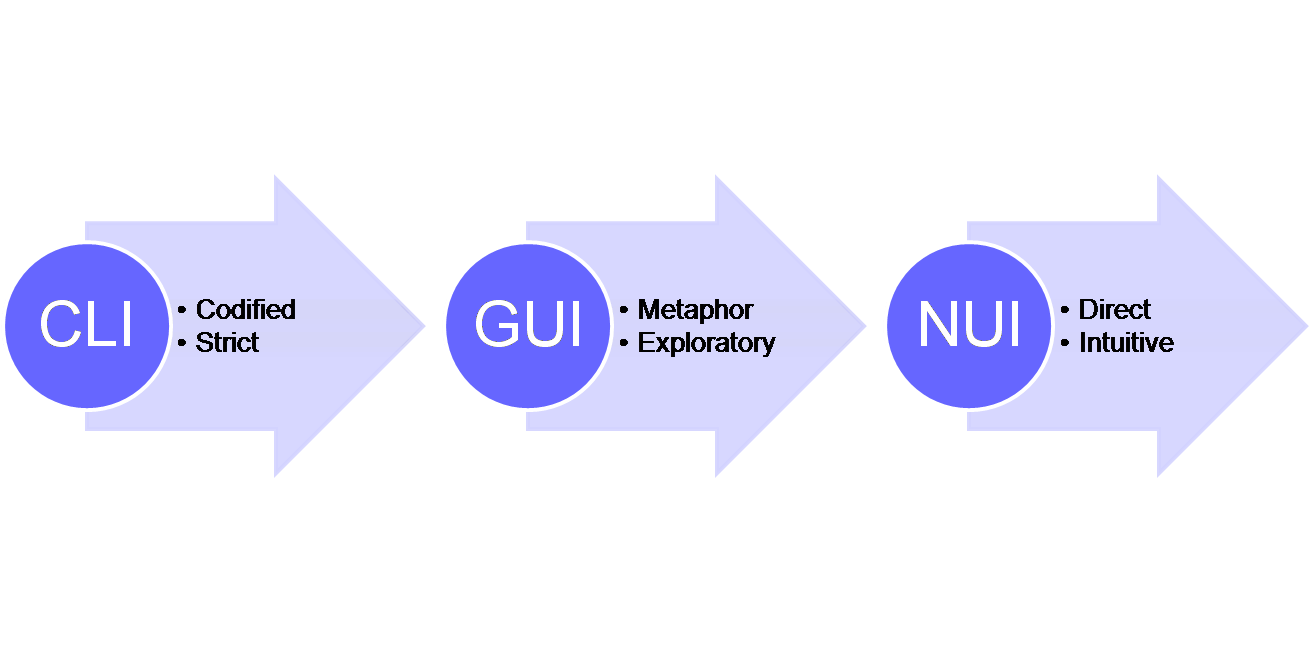
\includegraphics[width=1\textwidth]{images/nui.png}
\captionof{figure}{
Ewolucja interfejsów użytkownika\cite{nui}
}
\end{center}
\paragraph{}
Wiele nowych urządzeń próbuje implementować sterowanie interfejsem użytkownika za pomocą gestów (np. Microsoft Kinect\cite{kinect} lub sensor Leap Motion\cite{leap}), czy też za pomocą myśli (np. Emotiv\cite{emotiv}). Na rynku widać duże zainteresowanie nową formą kontroli urządzeniami, zwłaszcza tymi bardziej naturalnymi dla człowieka. Jedankaże obecnie są to głównie eksperymenty nowej technologii. Nie ma na rynku obecnie wypracowanego popularnego standardu dostępu w grupie NUI.
\newline
W branży filmowej oraz gier wideo narasta trend używania nowych technologii do rozszerzania doznań jakie otrzymuje odbiorca.
W kinach odbywają są coraz częściej projekcje filmów stworzonych w technologii trójwymiarowej. Natomiast w ostatnim czasie pojawią się sale kinowe pozwalające na projekcję filmów trójwymiarowych wraz z dodatkowymi elementami takimi jak: drganie foteli, wiatr, dym, woda\cite{cinema}. Jednakże w obecnej chwili taki format rozrywki jest dość drogi, gdyż wymaga specjalnie przygotowanej sali kinowej oraz okularów, które pozwalają tworzyć iluzję przestrzenną. 
\section*{Rozszerzona rzeczywistość}
\paragraph{}
Coraz bardziej popularne staje się pojęcie rozszerzonej rzeczywistości (ang. augmented reality). Jest to zbiór różnych technologii pozwalającej łączyć świat rzeczywisty z wirtualnym. Jest to jeszcze mało popularny sposób interakcji, lecz w ostatnim dziesięcioleciu rozwój (zarówno urządzeń jak i specjalistycznego oprogramowania) jest bardzo dynamiczny.
\newline
Pierwsze próby w tej dziedzinie odbywały się jeszcze w latach sześćdziesiątych amerykański naukowiec oraz artysta Myron Krueger prowadził badania nad wirtualną oraz rozszerzoną rzeczywistością. Jest on twórcą pojęcia środowiska responsywnego. ,,Jest to środowisko w którym działania użytkownika i odpowiada na nie w sposób przemyślany poprzez złożony system środków wizualnych i akustycznych, oraz dostosowuje się do powstałych w ten sposób nowych warunków środowiska\cite{kr}. Stworzył on interaktywne instalacje takie jak Glowflow\cite{glow}, Metaplay\cite{metaplay} oraz Videoplace\cite{videoplace}.
\begin{center}
\newpage
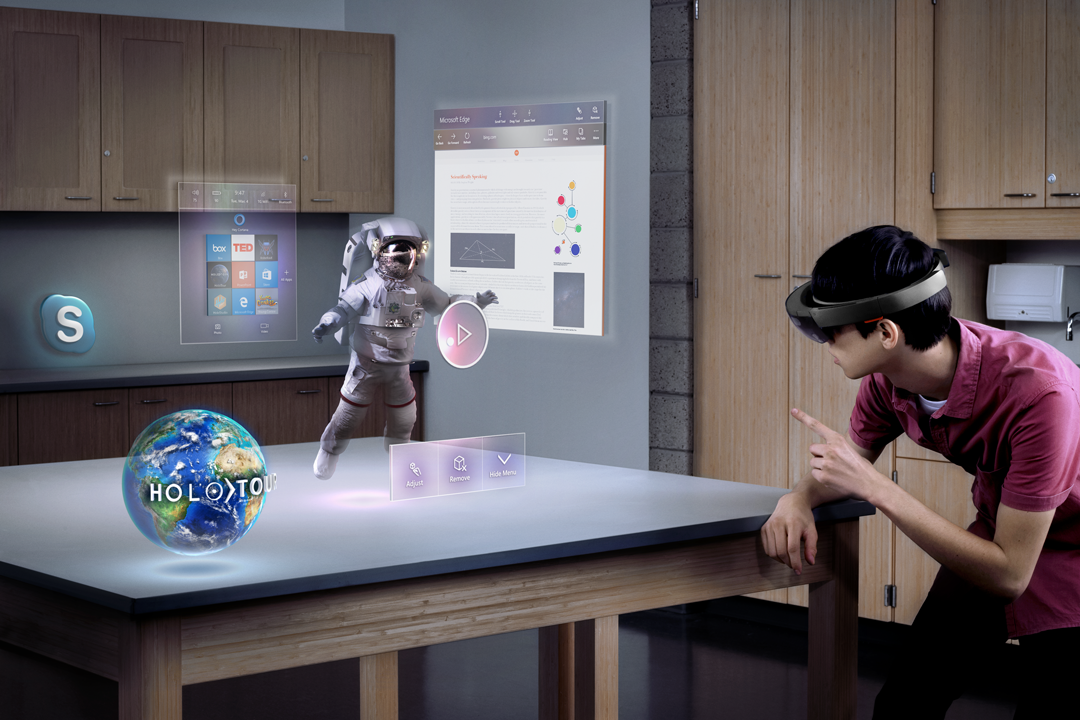
\includegraphics[width=1\textwidth]{images/hololens.png}
\captionof{figure}{
Wizualizacja Microsoft HoloLens\cite{holo2}
}
\end{center}
